\documentclass[12pt,a4paper]{report}

% ===================== PAKIETY =====================
\usepackage[utf8]{inputenc}
\usepackage[T1]{fontenc}
\usepackage[polish]{babel}
\usepackage{lmodern}
\usepackage{geometry}
\geometry{a4paper, margin=2.5cm}
\usepackage{graphicx}
\usepackage{listings}
\usepackage{xcolor}
\usepackage{caption}
\usepackage{hyperref}
\usepackage{fancyhdr}
\usepackage{titlesec}
\usepackage{amsmath}
\usepackage{amssymb}
\usepackage{booktabs}
\usepackage{float}
\usepackage{tikz}
\usetikzlibrary{arrows.meta, positioning}

% ===================== USTAWIENIA LISTINGS DLA SCL =====================
\lstdefinelanguage{SCL}{
    morekeywords={FUNCTION_BLOCK,END_FUNCTION_BLOCK,VAR_INPUT,VAR_OUTPUT,VAR,END_VAR,
    IF,THEN,ELSE,ELSIF,END_IF,CASE,OF,END_CASE,FOR,TO,DOWNTO,BY,DO,END_FOR,
    WHILE,END_WHILE,REPEAT,UNTIL,END_REPEAT,TRUE,FALSE,AND,OR,NOT,
    Int,Real,Bool,Time,Array,VERSION},
    morecomment=[l]{//},
    morestring=[b]",
    sensitive=false
}

\lstset{
    language=SCL,
    basicstyle=\ttfamily\footnotesize,
    keywordstyle=\color{blue}\bfseries,
    commentstyle=\color{green!50!black}\itshape,
    stringstyle=\color{orange},
    numbers=left,
    numberstyle=\tiny\color{gray},
    stepnumber=1,
    numbersep=8pt,
    breaklines=true,
    breakatwhitespace=false,
    frame=single,
    backgroundcolor=\color{gray!5},
    tabsize=2,
    showstringspaces=false
}

\pagestyle{fancy}
\fancyhf{}
\rhead{Sprawozdanie z projektu PLC}
\lhead{TIA Portal / SCL}
\rfoot{\thepage}

\begin{document}

% ===================== STRONA TYTUŁOWA =====================
\begin{titlepage}
    \centering

    % Tło – logo uczelni jako znak wodny (wgraj plik image.png do głównego katalogu projektu w Overleaf)
    \IfFileExists{image.png}{
        \begin{tikzpicture}[remember picture, overlay]
            \node[opacity=0.15, inner sep=0pt] at (current page.center) {
                \includegraphics[width=0.9\textwidth]{image.png}
            };
        \end{tikzpicture}
    }{}

    % Górny pasek
    \rule{\textwidth}{1pt}\\[0.1cm]
    {\large \scshape Akademia Marynarki Wojennej -- Wydział Mechaniczno Elektryczny}\\[0.2cm]
    \rule{\textwidth}{0.5pt}\\[1cm]

    % Tytuł
    {\huge \bfseries Sprawozdanie z projektu}\\[0.4cm]
    {\Large \textbf{Zaawansowane programowanie PLC}}\\[1.2cm]
    {\Large \textbf{Temat: } System sterowania automatycznym zbiornikiem mieszającym}\\[0.5cm]

    \rule{0.6\textwidth}{0.4pt}\\[0.6cm]

    % Autor
    {\large \textbf{Autor:}}\\[0.2cm]
    {\Large inż. Maciej Lutyński}\\[0.3cm]
    {\large Numer albumu: 24289}\\[0.3cm]
    {\large Grupa laboratoryjna: 212MCAI\_B}\\[0.8cm]

    \rule{0.6\textwidth}{0.4pt}\\[0.6cm]

    \vfill

    {\large \today}

\end{titlepage}

\thispagestyle{empty}
\newpage

\tableofcontents
\newpage

% =====================================================================
\chapter{Wstęp i cel projektu}
% =====================================================================

Celem projektu było opracowanie oraz uruchomienie w środowisku Siemens TIA Portal programu sterującego procesem technologicznym, który w sposób kompleksowy wykorzystuje podstawowe konstrukcje programistyczne stosowane w automatyce przemysłowej. Program napisano w języku strukturalnym SCL (ang. \textit{Structured Control Language}), zgodnym ze standardem IEC 61131-3.

Projekt miał spełniać następujące wytyczne programowe:

\begin{enumerate}
    \item Funkcje logiczne (AND, OR, NOT),
    \item Funkcje arytmetyczne,
    \item Instrukcje warunkowe (IF, CASE),
    \item Pętle (FOR),
    \item Timery (TON),
    \item Liczniki (CTU, CTD),
    \item Sterowanie zaworem analogowym,
    \item Detekcję zboczy sygnałów (R\_TRIG, F\_TRIG).
\end{enumerate}

Jako obiekt sterowania wybrano zbiornik technologiczny z automatycznym dozowaniem cieczy, mieszaniem oraz spustem — proces typowy dla przemysłu chemicznego, spożywczego i farmaceutycznego, w którym w naturalny sposób występują wszystkie wymienione wyżej elementy programistyczne.

% =====================================================================
\chapter{Opis procesu technologicznego}
% =====================================================================

Sterowany obiekt to zbiornik wyposażony w:

\begin{itemize}
    \item \textbf{czujnik poziomu analogowy} — sygnał wejściowy 0--27648 (odpowiadający zakresowi 0--100\% wypełnienia zbiornika),
    \item \textbf{zawór dozujący sterowany analogowo} — sygnał wyjściowy AO 0--27648, sterowany proporcjonalnie do uchybu regulacji,
    \item \textbf{pompę mieszającą} — sygnał dwustanowy (ON/OFF),
    \item \textbf{zawór spustowy} — sygnał dwustanowy (ON/OFF),
    \item wejścia operatorskie: \texttt{Start}, \texttt{Stop}, \texttt{Kasuj\_Alarm},
    \item wejście awarii zewnętrznej (np. zabezpieczenie termiczne silnika mieszadła).
\end{itemize}

Cykl pracy zbiornika przebiega w czterech głównych etapach, zaimplementowanych jako maszyna stanów:

\begin{enumerate}
    \item \textbf{IDLE} (stan 0) — oczekiwanie na sygnał start przy spełnionych warunkach zezwolenia,
    \item \textbf{NAPEŁNIANIE} (stan 1) — otwarcie zaworu dozującego proporcjonalnie do różnicy poziomu zadanego i rzeczywistego, aż do osiągnięcia poziomu zadanego,
    \item \textbf{MIESZANIE} (stan 2) — załączenie pompy mieszającej na czas zadany przez timer,
    \item \textbf{SPUST} (stan 3) — otwarcie zaworu spustowego na zadany czas,
    \item \textbf{ZAKOŃCZONO} (stan 4) — inkrementacja licznika wykonanych cykli (batchy) i powrót do stanu IDLE.
\end{enumerate}

Dodatkowo program rejestruje historię 10 ostatnich pomiarów poziomu i wylicza z nich wartość średnią, a każda zarejestrowana awaria zmniejsza licznik zliczający w dół, sygnalizujący potrzebę przeglądu serwisowego.

% =====================================================================
\chapter{Struktura programu w TIA Portal}
% =====================================================================

Program zrealizowano w postaci pojedynczego bloku funkcyjnego (Function Block) \texttt{FB\_ZbiornikMieszajacy}, wywoływanego cyklicznie w bloku organizacyjnym \texttt{OB1 (Main)} z powiązaną instancją danych \texttt{"FB\_Zbiornik Mieszajacy\_DB"}.

\section{Interfejs bloku}

\begin{table}[H]
\centering
\caption{Zmienne wejściowe bloku FB\_ZbiornikMieszajacy}
\begin{tabular}{@{}lll@{}}
\toprule
\textbf{Nazwa} & \textbf{Typ} & \textbf{Opis} \\
\midrule
Start & Bool & Przycisk uruchomienia cyklu \\
Stop & Bool & Przycisk zatrzymania cyklu \\
Kasuj\_Alarm & Bool & Kasowanie sygnalizacji awarii \\
Awaria\_Zewn & Bool & Sygnał awarii z instalacji \\
Poziom\_Analog\_In & Int & Surowy sygnał z czujnika poziomu (0--27648) \\
Poziom\_Zadany & Real & Wartość zadana poziomu w \% \\
Czas\_Mieszania & Time & Nastawa czasu mieszania \\
Czas\_Spustu & Time & Nastawa czasu spustu \\
\bottomrule
\end{tabular}
\end{table}

\begin{table}[H]
\centering
\caption{Zmienne wyjściowe bloku FB\_ZbiornikMieszajacy}
\begin{tabular}{@{}lll@{}}
\toprule
\textbf{Nazwa} & \textbf{Typ} & \textbf{Opis} \\
\midrule
Zawor\_Dozujacy\_AO & Int & Wyjście analogowe sterujące zaworem \\
Pompa\_Mieszajaca & Bool & Sterowanie pompą mieszającą \\
Zawor\_Spustowy & Bool & Sterowanie zaworem spustowym \\
Lampka\_Alarm & Bool & Sygnalizacja awarii \\
Lampka\_Praca & Bool & Sygnalizacja pracy procesu \\
Licznik\_Cykli & Int & Liczba wykonanych cykli (batchy) \\
Stan\_Procesu & Int & Aktualny stan maszyny stanów (0--4) \\
Poziom\_Procent & Real & Poziom przeliczony na \% \\
Srednia\_Poziomu & Real & Średnia z 10 ostatnich próbek \\
Serwis\_Wymagany & Bool & Sygnał żądania przeglądu serwisowego \\
\bottomrule
\end{tabular}
\end{table}

\section{Zmienne wewnętrzne}

Wewnątrz bloku zadeklarowano instancje bloków standardowych: \texttt{R\_TRIG}, \texttt{F\_TRIG}, \texttt{TON} (dwie instancje), \texttt{CTU} oraz \texttt{CTD}, a także tablicę dziesięcioelementową \texttt{Historia\_Poziomu : Array[1..10] of Real} przechowującą historię próbek poziomu wykorzystywaną do obliczania wartości średniej.

% =====================================================================
\chapter{Omówienie kodu źródłowego}
% =====================================================================

Poniżej przedstawiono realizację poszczególnych wymaganych elementów programistycznych wraz z fragmentami kodu SCL oraz odpowiadającymi zrzutami ekranu z edytora TIA Portal.

\section{Detekcja zboczy}

Wykrywanie zbocza narastającego na sygnale \texttt{Start} oraz zbocza opadającego na sygnale \texttt{Stop} zrealizowano przy użyciu standardowych bloków \texttt{R\_TRIG} i \texttt{F\_TRIG}:

\begin{lstlisting}
#Start_Trig(CLK := #Start);
#Stop_Trig(CLK := #Stop);
\end{lstlisting}

Wyjście \texttt{Start\_Trig.Q} generuje pojedynczy impuls trwający jeden cykl programu w momencie zbocza narastającego sygnału Start, co zabezpiecza przed wielokrotnym uruchomieniem cyklu przy przytrzymanym przycisku. Analogicznie \texttt{Stop\_Trig.Q} wykorzystywane jest do natychmiastowego, jednorazowego resetu procesu do stanu IDLE.

\begin{figure}[H]
\centering
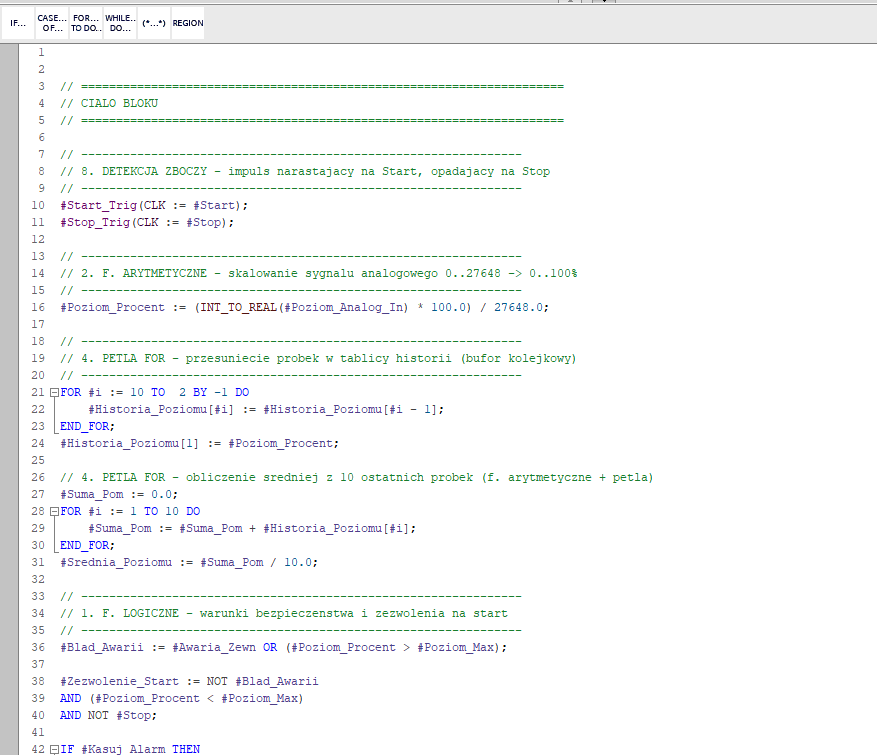
\includegraphics[width=0.95\linewidth]{images/KOD_cz1.png}
\caption{Fragment kodu — detekcja zboczy, skalowanie sygnału analogowego oraz pętle FOR}
\label{fig:kod1}
\end{figure}

\section{Funkcje arytmetyczne}

Skalowanie sygnału z modułu wejść analogowych (zakres 0--27648) do wartości procentowej realizuje poniższa instrukcja:

\begin{lstlisting}
#Poziom_Procent := (INT_TO_REAL(#Poziom_Analog_In) * 100.0) / 27648.0;
\end{lstlisting}

Dodatkowo funkcje arytmetyczne wykorzystano przy obliczaniu uchybu regulacji (różnica poziomu zadanego i rzeczywistego), przeliczaniu procentowego otwarcia zaworu na wartość surową sygnału AO oraz przy sumowaniu próbek historii w celu wyznaczenia wartości średniej.

\section{Pętle FOR}

Zaimplementowano dwie pętle FOR. Pierwsza realizuje przesunięcie próbek w buforze kołowym (najstarsza próbka jest usuwana, nowa wstawiana na początek tablicy):

\begin{lstlisting}
FOR #i := 10 DOWNTO 2 DO
    #Historia_Poziomu[#i] := #Historia_Poziomu[#i - 1];
END_FOR;
#Historia_Poziomu[1] := #Poziom_Procent;
\end{lstlisting}

Druga pętla sumuje zawartość tablicy w celu obliczenia średniej kroczącej z 10 ostatnich pomiarów:

\begin{lstlisting}
#Suma_Pom := 0.0;
FOR #i := 1 TO 10 DO
    #Suma_Pom := #Suma_Pom + #Historia_Poziomu[#i];
END_FOR;
#Srednia_Poziomu := #Suma_Pom / 10.0;
\end{lstlisting}

\section{Funkcje logiczne}

Warunki bezpieczeństwa oraz zezwolenia na start cyklu zbudowano z operatorów logicznych AND, OR, NOT:

\begin{lstlisting}
#Blad_Awarii := #Awaria_Zewn OR (#Poziom_Procent > #Poziom_Max);

#Zezwolenie_Start := NOT #Blad_Awarii
                 AND (#Poziom_Procent < #Poziom_Max)
                 AND NOT #Stop;
\end{lstlisting}

\begin{figure}[H]
\centering
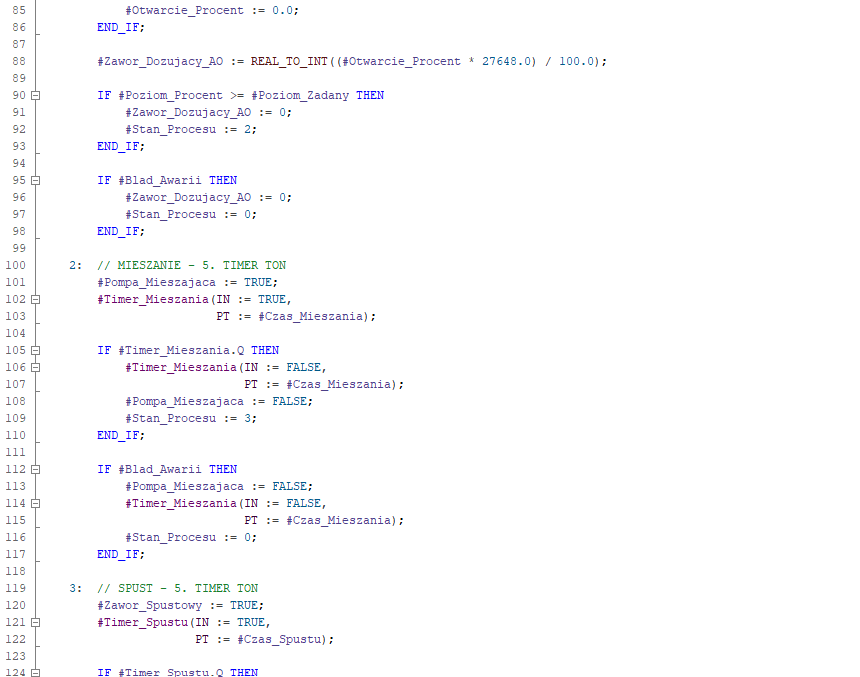
\includegraphics[width=0.95\linewidth]{images/kod_cz3.png}
\caption{Fragment kodu — funkcje logiczne, obsługa zbocza Stop oraz początek maszyny stanów CASE}
\label{fig:kod3}
\end{figure}

\section{Instrukcje warunkowe — maszyna stanów}

Główną logikę sterującą procesem zrealizowano w postaci instrukcji \texttt{CASE}, w której każdy stan odpowiada jednemu etapowi procesu technologicznego (IDLE, NAPEŁNIANIE, MIESZANIE, SPUST, ZAKOŃCZONO). Dodatkowo w obrębie poszczególnych gałęzi zastosowano instrukcje \texttt{IF...THEN...ELSE} do regulacji proporcjonalnej otwarcia zaworu oraz ograniczenia zakresu sterowania do 0--100\%.

\begin{figure}[H]
\centering
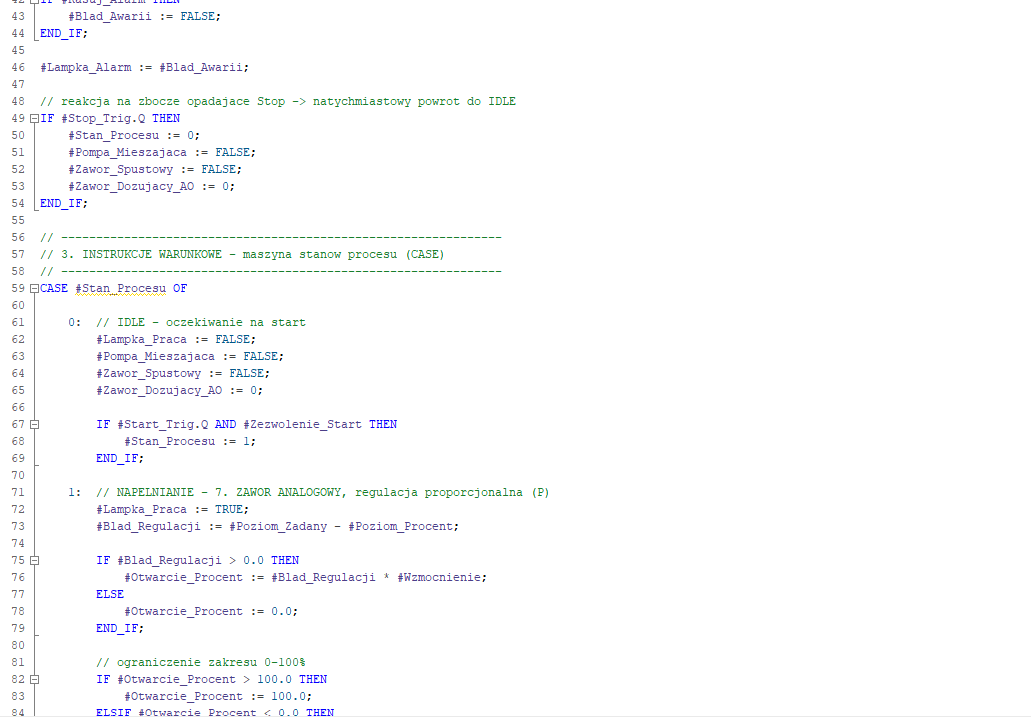
\includegraphics[width=0.95\linewidth]{images/KOD_cz2.png}
\caption{Fragment kodu — regulacja proporcjonalna zaworu, stan MIESZANIE i SPUST (timery TON)}
\label{fig:kod2}
\end{figure}

\section{Timery}

Do odmierzania czasu mieszania oraz czasu spustu wykorzystano dwie niezależne instancje bloku opóźnienia załączenia \texttt{TON}:

\begin{lstlisting}
#Timer_Mieszania(IN := TRUE, PT := #Czas_Mieszania);
IF #Timer_Mieszania.Q THEN
    ...
END_IF;
\end{lstlisting}

\section{Liczniki}

Zliczanie wykonanych cykli technologicznych (batchy) zrealizowano licznikiem zliczającym w górę \texttt{CTU}, natomiast odliczanie do przeglądu serwisowego — licznikiem zliczającym w dół \texttt{CTD}, kasowanym sygnałem \texttt{Kasuj\_Alarm}:

\begin{lstlisting}
#Licznik_Batch(CU := TRUE, R := FALSE, PV := 9999);
#Licznik_Cykli := #Licznik_Batch.CV;

#Licznik_Serwis(CD := #Blad_Awarii, LD := #Kasuj_Alarm, PV := 5);
#Serwis_Wymagany := #Licznik_Serwis.Q;
\end{lstlisting}

\begin{figure}[H]
\centering
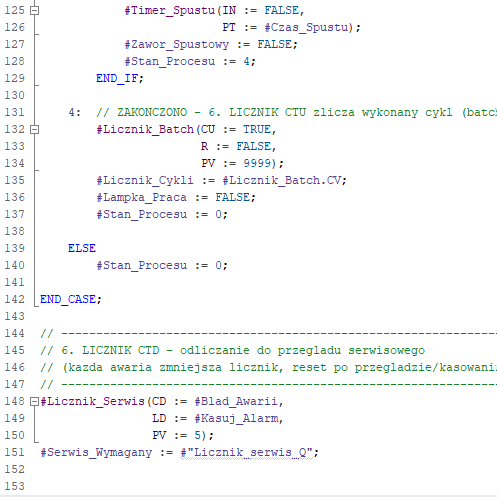
\includegraphics[width=0.95\linewidth]{images/kod_cz4.png}
\caption{Fragment kodu — stan ZAKOŃCZONO (licznik CTU) oraz licznik serwisowy CTD}
\label{fig:kod4}
\end{figure}

\section{Sterowanie zaworem analogowym}

W stanie NAPEŁNIANIE zaimplementowano prosty regulator proporcjonalny (P), którego wyjście po ograniczeniu do zakresu 0--100\% jest przeliczane na wartość surową sygnału wyjściowego AO:

\begin{lstlisting}
#Blad_Regulacji := #Poziom_Zadany - #Poziom_Procent;

IF #Blad_Regulacji > 0.0 THEN
    #Otwarcie_Procent := #Blad_Regulacji * #Wzmocnienie;
ELSE
    #Otwarcie_Procent := 0.0;
END_IF;

IF #Otwarcie_Procent > 100.0 THEN
    #Otwarcie_Procent := 100.0;
ELSIF #Otwarcie_Procent < 0.0 THEN
    #Otwarcie_Procent := 0.0;
END_IF;

#Zawor_Dozujacy_AO := REAL_TO_INT((#Otwarcie_Procent * 27648.0) / 100.0);
\end{lstlisting}

% =====================================================================
\chapter{Uruchomienie i testowanie programu}
% =====================================================================

\section{Metodyka testów}

Program został przetestowany bez użycia fizycznego sterownika, z wykorzystaniem symulatora \textbf{PLCSIM} zintegrowanego z TIA Portal. Weryfikację poprawności działania przeprowadzono poprzez podgląd w trybie monitorowania (\textit{monitoring mode}) bezpośrednio na graficznym symbolu wywołania bloku funkcyjnego w \texttt{OB1}, gdzie w czasie rzeczywistym widoczne są wartości wszystkich zmiennych wejściowych i wyjściowych instancji \texttt{"FB\_Zbiornik Mieszajacy\_DB"}. Wartości sygnałów wejściowych (poziom, wartość zadana, sygnały Start/Stop) wymuszano ręcznie w celu weryfikacji poprawności przejść pomiędzy poszczególnymi stanami procesu.

\section{Scenariusze testowe i wyniki}

\subsection*{Test 1 — stan spoczynkowy (IDLE)}

Przy braku wymuszenia sygnału Start oraz zerowym poziomie w zbiorniku (\texttt{Poziom\_Analog\_In = 0}) program pozostaje w stanie \texttt{Stan\_Procesu = 0}. Wszystkie wyjścia sterujące (pompa, zawór spustowy, zawór dozujący, lampka pracy) są nieaktywne, co potwierdza poprawną inicjalizację i logikę stanu IDLE.

\begin{figure}[H]
\centering
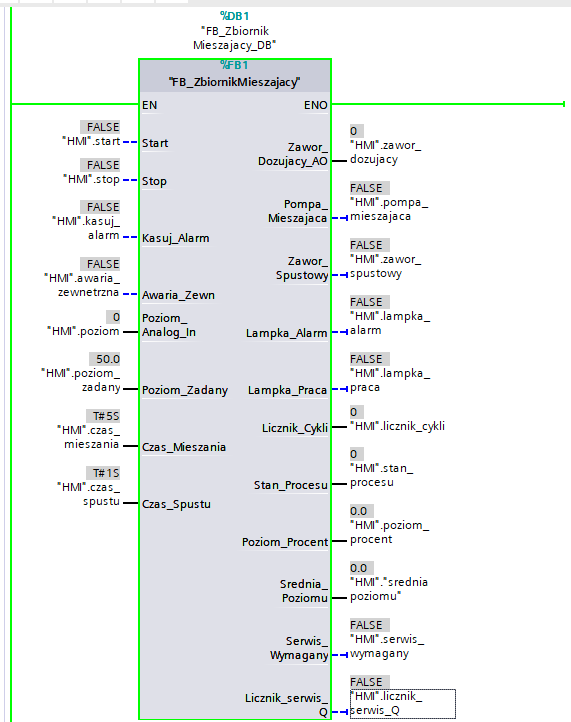
\includegraphics[width=0.7\linewidth]{images/FB_cz1.png}
\caption{Monitoring instancji bloku — stan spoczynkowy IDLE (Stan\_Procesu = 0)}
\label{fig:fb1}
\end{figure}

\subsection*{Test 2 — przejście do stanu NAPEŁNIANIE}

Po wymuszeniu impulsu na wejściu \texttt{Start} program przeszedł do stanu \texttt{Stan\_Procesu = 1} (NAPEŁNIANIE). Przy dużym uchybie regulacji (poziom zadany 50\%, poziom rzeczywisty 0\%) regulator proporcjonalny wysterował zawór dozujący do wartości maksymalnej — \texttt{Zawor\_Dozujacy\_AO = 27648} (100\% otwarcia), co potwierdza poprawne działanie ograniczenia zakresu regulacji (\textit{clamping}) oraz sygnalizacji pracy (\texttt{Lampka\_Praca = TRUE}).

\begin{figure}[H]
\centering
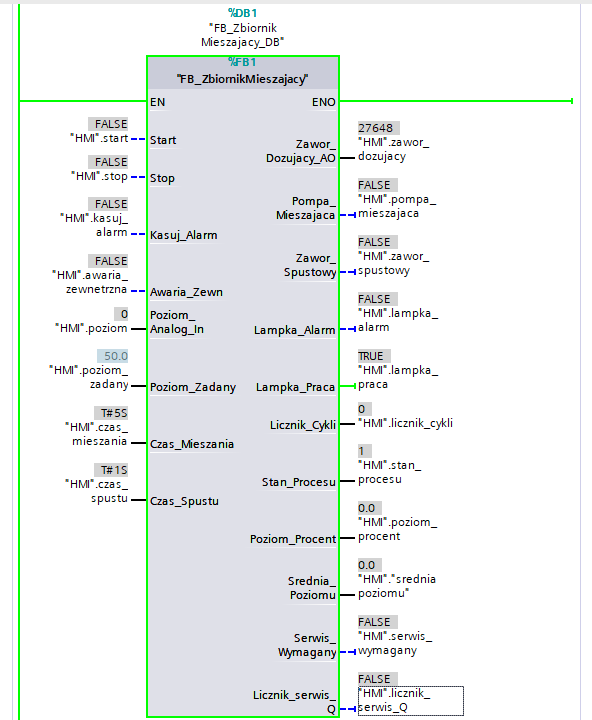
\includegraphics[width=0.7\linewidth]{images/FB_cz2.png}
\caption{Monitoring instancji bloku — stan NAPEŁNIANIE, pełne otwarcie zaworu przy dużym uchybie}
\label{fig:fb2}
\end{figure}

\subsection*{Test 3 — weryfikacja skalowania i uśredniania poziomu}

Przy wymuszeniu sygnału \texttt{Poziom\_Analog\_In = 6000} program poprawnie przeliczył wartość na jednostki procentowe zgodnie ze wzorem skalującym:
\[
Poziom\_Procent = \frac{6000 \cdot 100}{27648} \approx 21{,}70\%
\]
co zostało potwierdzone odczytem \texttt{Poziom\_Procent = 21.70139} widocznym na zrzucie ekranu. Wartość \texttt{Srednia\_Poziomu} przyjęła identyczną wartość, co jest zgodne z oczekiwaniami przy pierwszym cyklu wypełniania tablicy historii (wszystkie 10 elementów bufora zawiera jeszcze wartości domyślne z tej samej próbki).

\begin{figure}[H]
\centering
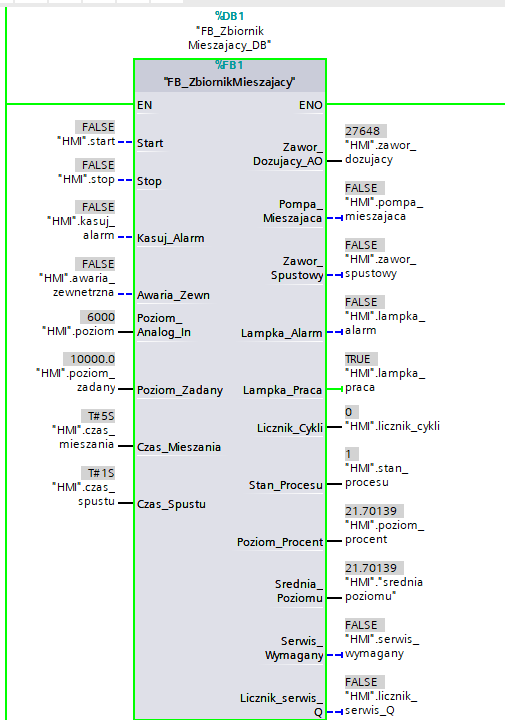
\includegraphics[width=0.7\linewidth]{images/FB_cz3.png}
\caption{Monitoring instancji bloku — poprawne przeliczenie sygnału analogowego na wartość procentową}
\label{fig:fb3}
\end{figure}

\subsection*{Test 4 — powrót do stanu IDLE}

Po wymuszeniu sygnału \texttt{Stop} (zbocze opadające) program natychmiast wrócił do stanu \texttt{Stan\_Procesu = 0}, wyzerował wyjście zaworu dozującego oraz wyłączył sygnalizację pracy, co potwierdza poprawność obsługi przerwania cyklu w dowolnym jego momencie.

\begin{figure}[H]
\centering
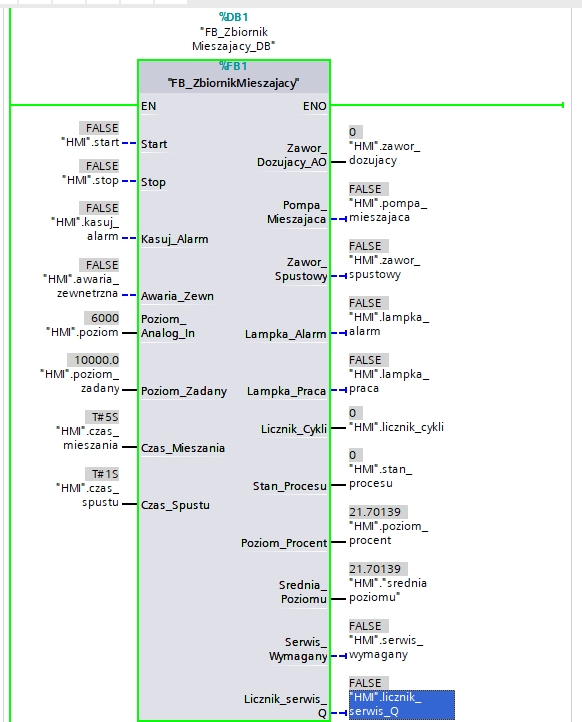
\includegraphics[width=0.7\linewidth]{images/FB_cz4.png}
\caption{Monitoring instancji bloku — powrót do stanu IDLE po zboczu opadającym sygnału Stop}
\label{fig:fb4}
\end{figure}

\section{Uwagi z testów}

Podczas testów zaobserwowano, że w niektórych przebiegach testowych parametr \texttt{Poziom\_Zadany} był wymuszany wartością znacznie przekraczającą zakres 0--100 (np. 10000.0), co nie odpowiada założeniu przyjętemu w projekcie (wartość zadana powinna być podawana w jednostkach procentowych). W takim przypadku uchyb regulacji jest zawsze bardzo duży, a regulator proporcjonalny utrzymuje zawór w pełnym otwarciu niezależnie od aktualnego poziomu — jest to zachowanie zgodne z zaimplementowanym ograniczeniem zakresu sterowania (\textit{clamping do 100\%}), a nie błąd programu. Wniosek ten wskazuje na konieczność dodania w przyszłej wersji programu kontroli poprawności zakresu wartości zadawanych przez operatora (walidacja wejścia \texttt{Poziom\_Zadany} do przedziału 0--100).

% =====================================================================
\chapter{Wnioski}
% =====================================================================

\begin{enumerate}
    \item Zaimplementowany program w pełni realizuje wszystkie założone wymagania projektowe: funkcje logiczne, funkcje arytmetyczne, instrukcje warunkowe, pętle, timery, liczniki, sterowanie zaworem analogowym oraz detekcję zboczy sygnałów.
    \item Zastosowanie maszyny stanów opartej na instrukcji CASE pozwoliło na czytelne i łatwe w rozbudowie zaprogramowanie sekwencji technologicznej.
    \item Testy przeprowadzone w środowisku symulacyjnym PLCSIM z podglądem online na bloku wywołania potwierdziły poprawność działania wszystkich kluczowych mechanizmów programu — skalowania sygnału analogowego, regulacji proporcjonalnej zaworu, przejść między stanami procesu oraz reakcji na sygnały Start/Stop.
    \item Zidentyfikowano potencjalny obszar do rozwoju programu — walidację zakresu wartości zadawanych przez operatora, co zwiększyłoby odporność aplikacji na błędne dane wejściowe.
    \item W dalszym rozwoju projektu warto rozważyć zastąpienie regulatora proporcjonalnego (P) regulatorem PI w celu eliminacji uchybu ustalonego oraz dodanie wizualizacji HMI umożliwiającej operatorowi łatwiejsze zadawanie parametrów procesu.
\end{enumerate}

% =====================================================================
\appendix
\chapter{Pełny kod źródłowy}
% =====================================================================

\section{Blok funkcyjny FB\_ZbiornikMieszajacy}
\lstinputlisting[language=SCL]{kod/FB_ZbiornikMieszajacy.scl}

\section{Wywołanie w OB1 (Main)}
\lstinputlisting[language=SCL]{kod/OB1_Main_wywolanie.scl}

\end{document}
